\chapter{系統架構與實作}

    本研究所設計之系統,利用超聲波對麥克風造成的非線性響應輸出,與主動式噪音控制消除高關聯度噪音等特性。
嘗試解決在部署麥克風干擾器的場域裡,無法取得有效聲學紀錄的問題。
同時借鏡密碼系統的機密性與不可否認性,發展一套於會談結束後,以其為基礎的會談錄音存取控制機制。
透過上述機制的結合,能夠使在部署超音波麥克風干擾器的會談情境中,於會談結束後,允許特定參與者得以取得有效之聲音記錄。


\section{系統架構}

\begin{figure}[H]
    \centering
    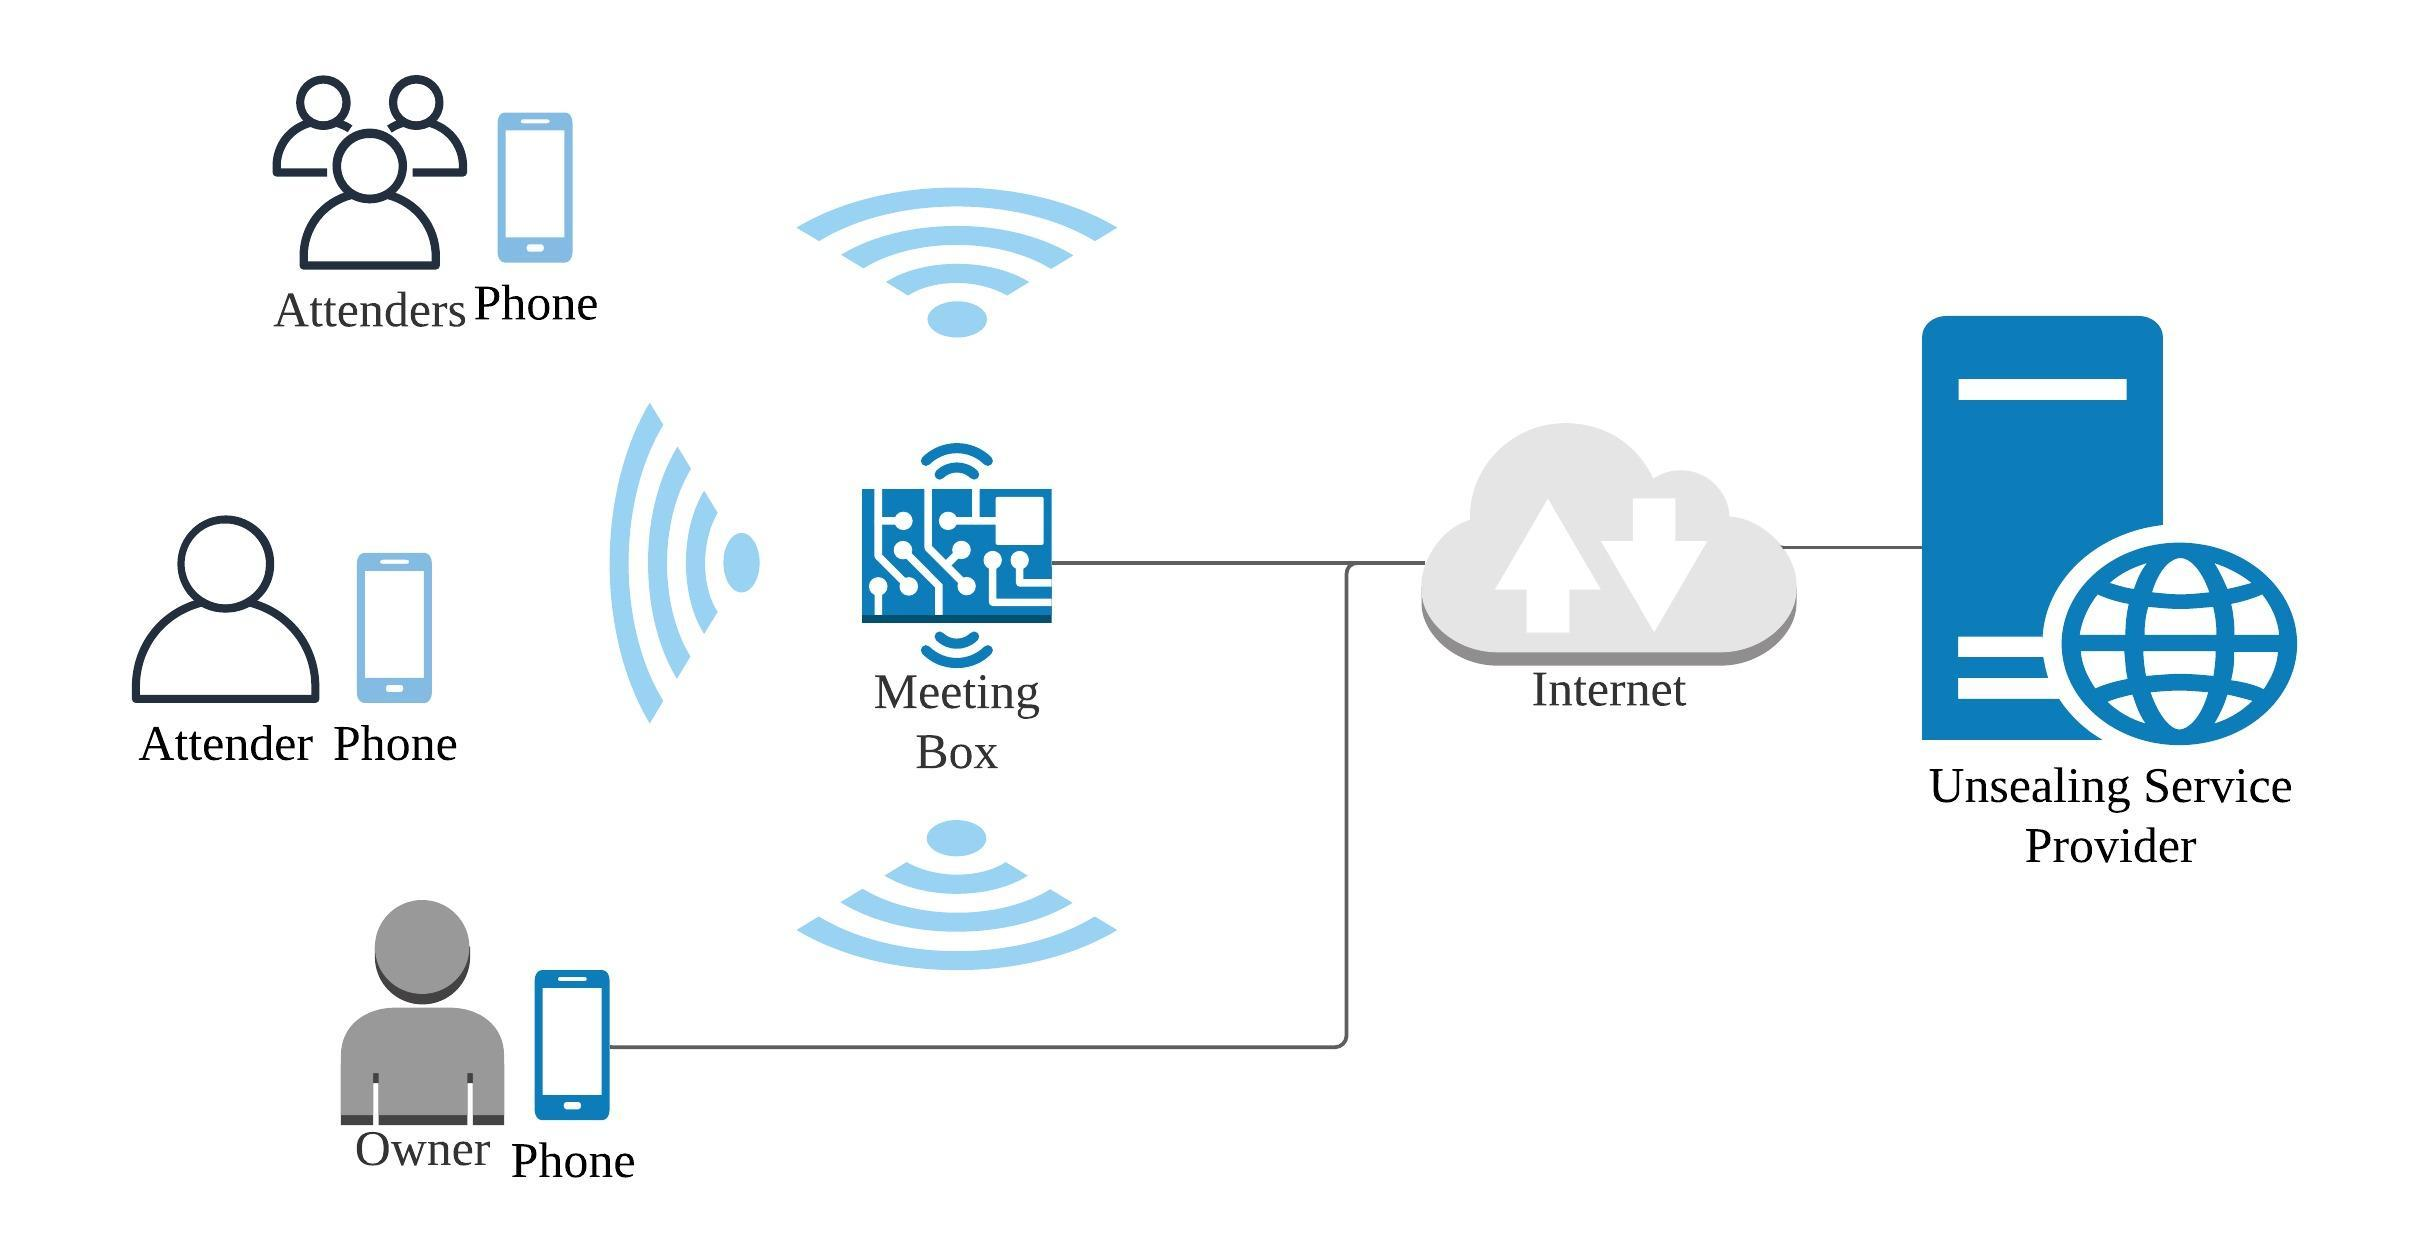
\includegraphics[width=0.8\textwidth]{single-owner-architecture}
    \caption{單一 Owner 系統架構圖}
    \label{fig.s-o-arch}
\end{figure}

    本系統由 $MeetingBox$、$Server$ 以及會談參與者 ($Attender$) 所組成。
$Attender$ 於 $MeetingBox$ 的周圍進行會談 ({\it Meeting Session}),
$MeetingBox$ 於會談進行間開啟超聲波麥克風干擾器,
因此鄰近的麥克風或周邊的聲音記錄裝置,都將因受到干擾而失效,$Attender$ 無法有效記錄會談的聲音內容。

    $MeetingBox$ 於會談進行中持續紀錄聲音,內容為受到超聲波麥克風干擾器干擾的會談錄音 ($REC_{J}$)。
於會談結束後,受超聲波麥克風干擾器干擾的會談聲音記錄 ($REC_{J}$) 將透過本研究所設計的「解封」 (Unseal) 機制,
使會談參與者 ($Attender$) 中的會談擁有者 ($Owner$),得以取得已解封 (Unsealed) 的有效聲音記錄 ($REC_{rev}$)。

    各會談的 $Attender$ 僅定義於當次會談,每次參與會談的 $Attender$ 可為不同群體。
$Attender$ 透過 $MeetingBox$ 上的控制介面與其互動,進而控制本研究所設計系統的生命週期。


\subsection{$Attender$}

    會談參與者 ($Attender$) 為一集合,代表所有當次會談 ({\it Meeting Session}) 的參與者。
$Attender$ 包含 $Owner$,為 $Owner$ 的超集合。其餘非 $Owner$ 的 $Attender$ 視為 $not$ $Owner$ $Attender$。
$Attender$ 可以透過 $MeetingBox$ 上的控制介面與其互動,來控制會議的開始與終止,本研究以實體按鈕為例。

    $Attender$ 受到 $MeetingBox$ 中的超聲波麥克風干擾器的干擾,使得隨身的麥克風或聲音記錄裝置,
都將因受到干擾而失效,無法有效記錄會談內容。例如:智慧型手機、智慧手錶、筆電、平板、智慧喇叭等。


\subsection{$Owner$}

\begin{figure}[H]
    \centering
    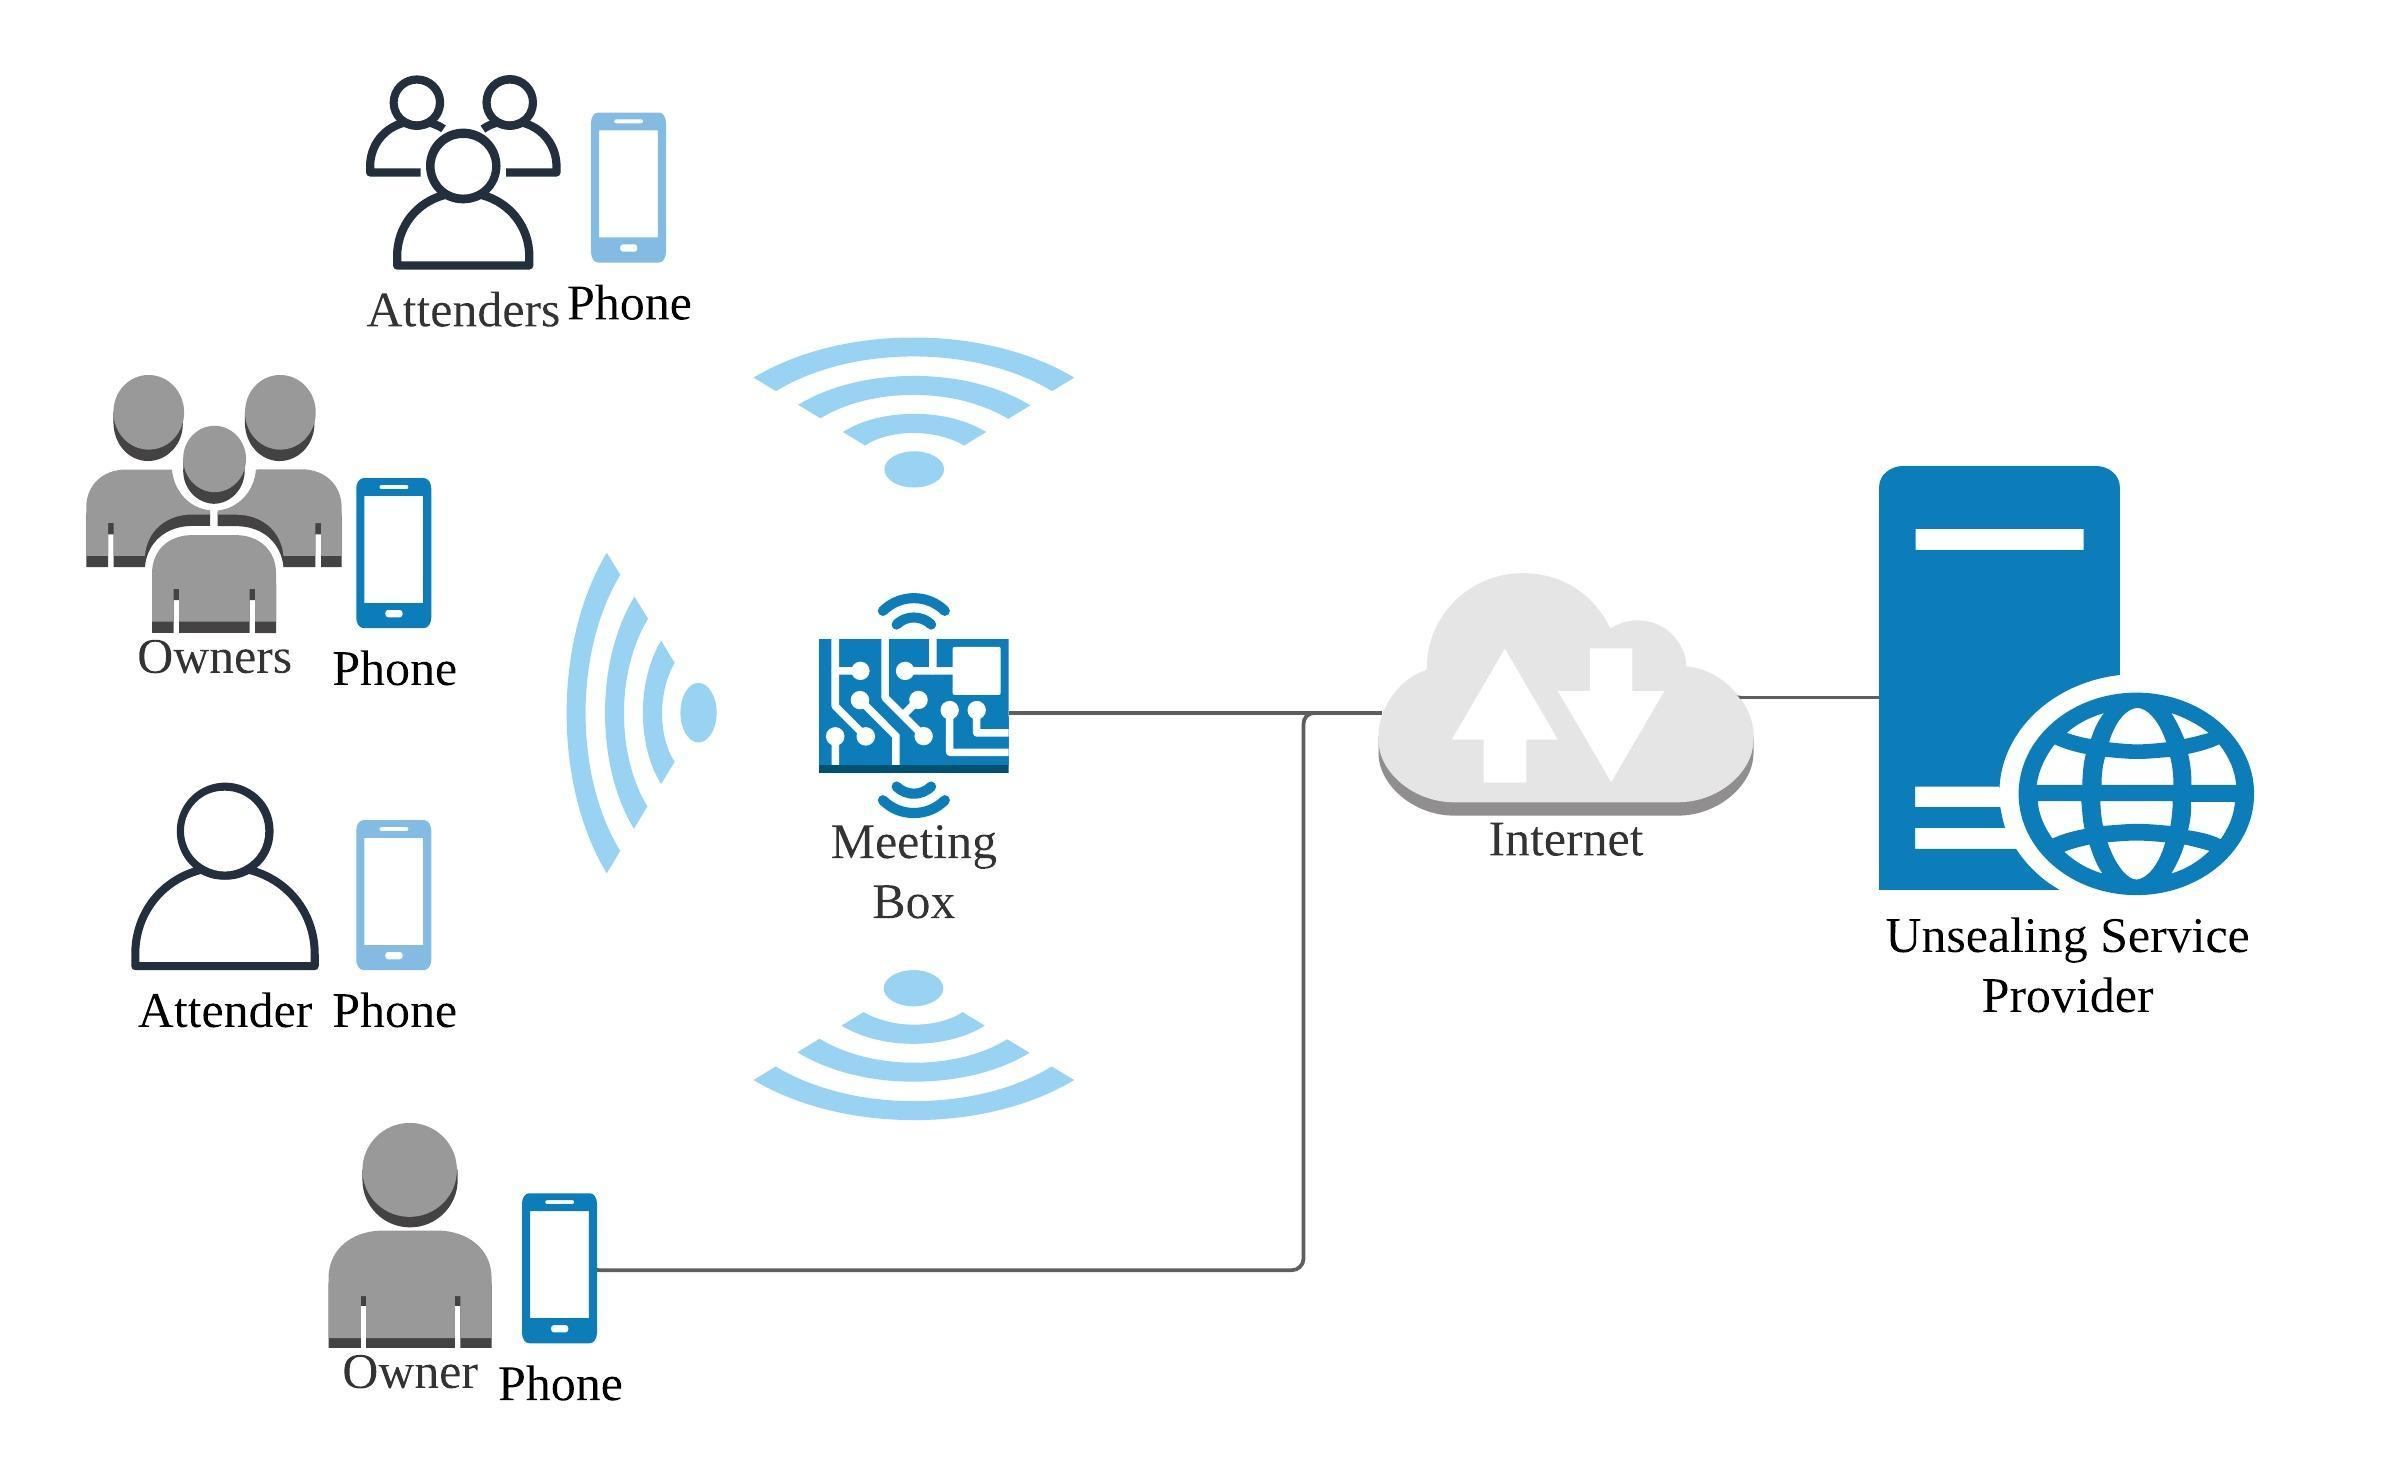
\includegraphics[width=0.8\textwidth]{multi-owner-architecture}
    \caption{多 Owner 系統架構圖}
    \label{fig.m-o-arch}
\end{figure}

    會談擁有者 ($Owner$) 屬於 $Attender$,為 $Attender$ 的子集合,
$Owner$ 定義為 $Attender$ 中的特權角色。$Owner$ 如未執行本研究所設計的系統機制「註冊會議擁有者」 (Register Owner),
則視為 $not$ $Owner$ $Attender$。 $Owner$ 於會談 ({\it Meeting Session}) 結束後,
有能力決定是否「解封」 (Unseal) 會談聲音記錄,並獲取已解封 (Unsealed) 的有效聲音記錄 ($REC_{rev}$)。

    $Owner$ 可以是一或多人。當會談中只有一個 $Owner$ 時,為 {\it Single Owner Meeting Session} 情境,
系統架構如圖 \ref{fig.s-o-arch}。當會談中多於一個 $Owner$ 時,為 {\it Multi Owner Meeting Session} 情境,
系統架構如圖 \ref{fig.m-o-arch} 所示。

    $Owner$ 持有智慧型裝置,透過其與 $MeetingBox$ 互動,獲取 $MeetingBox$ 上的資訊,並有能力於會談進行中、會談結束後,
與 $Server$ 持續通訊,執行本研究所設計的系統機制「註冊會議擁有者」 (Register Owner) 與「解封」 (Unseal)。

    上述 $Owner$ 獲取 $MeetingBox$ 資訊的方法,本研究以掃描 QR Code 為例。


\subsection{$MeetingBox$}

    $MeetingBox$ 為本研究所設計系統核心組成要件的終端,部署於會談 ({\it Meeting Session}) 的場域,
與會議參與者 ($Attender$) 實體接觸。透過與 $Attender$ 的互動,成為觸發會談生命週期改變事件的控制核心。
同時也作為系統主要資料 ($REC_{J}$、$REC_{N}$) 的輸入來源。
在本研究的設計中,一組 $MeetingBox$ 僅能同時間處理一場會談的進行。

    本研究所設計的 $MeetingBox$ 裝置包含下列組件:

    \begin{enumerate}
        \item 超音波麥克風干擾器:\\
            使用偽隨機數產生亂數頻率的超音波,於會談進行中開啟。用於干擾鄰近周圍含有麥克風的裝置,使其無法有效記錄會談內容。

        \item 錄音麥克風:\\
            用於紀錄會談的聲音內容 ($REC_{J}$),與產生超聲波麥克風干擾器於麥克風的響應輸出 ($REC_{N}$)

        \item 物理控制介面:\\
            提供 $Attender$ 操作與 $MeetingBox$ 互動,獲得外部觸發事件。本研究實做以實體按鈕為例。

        \item 人機互動介面:\\
            用於傳遞會談的 meta data 與系統狀態提示給 $Attender$,本研究實做以 QR Code 搭配螢幕顯示為例。

        \item 運算控制核心與網路介面:\\
            周邊裝置控制與邏輯運算核心,用於加密,與 Server 通訊等運算工作。
    \end{enumerate}


\subsection{$Server$}



\section{符號定義}

    本研究設計之系統所使用符號與其意義如表 \ref{table:tab.symbol} 所示。

\begin{table}[H]
    \centering
    \caption{符號定義表}
    \label{table:tab.symbol}
    \begin{tabular}{ c c }
        \hline
        \bf{符號} & \bf{釋義} \\
        \hline
        $Attender_{m}$ & 會議參與者 $Attender$ 中,任意特定一位 \\
        $Owner_{n}$    & 會議參與者 $Owner$ 中,任意特定一位 \\
        $REC_{J}$      & 已被超聲波麥克風干擾器干擾的會談之聲音記錄 \\
        $REC_{N}$      & 超聲波麥克風干擾器於麥克風的響應輸出之聲音記錄 \\
        $REC_{rev}$    & 解封後 (Unsealed) 的會談聲音記錄 \\
        $time_{Max}$   & 會談進行時間長度的最大值、$REC_{N}$ 的時間長度 \\
    \end{tabular}
\end{table}

\section{系統流程}

\section{系統機制}

\subsection{錄音存取控制與解密}

\subsection{主動式噪音控制}

\subsection{樣本對齊}

\section{系統實作}